\documentclass[10pt]{article}

\usepackage[letterpaper,margin=0.85in]{geometry}
\usepackage{amsmath,amssymb}
\usepackage{booktabs}
\usepackage{graphicx}
\usepackage{microtype}
\usepackage[numbers,sort&compress]{natbib}
\usepackage{enumitem}
\usepackage{xcolor}
\usepackage{hyperref}
\usepackage{caption}
\usepackage{subcaption}
\usepackage{array}
\usepackage{tabularx}
\usepackage{tikz}
\usetikzlibrary{arrows.meta,positioning,fit,backgrounds}

\definecolor{keystoneblue}{HTML}{163B64}
\hypersetup{colorlinks=true,linkcolor=keystoneblue,citecolor=keystoneblue,urlcolor=keystoneblue,
  pdftitle={KEYSTONE: Auditable Dispute-Key Availability for Encrypted AI Rollups},
  pdfauthor={Zubaer Mahmood Zubraj},
  pdfkeywords={dispute-key availability, threshold decryption, encrypted rollups, readiness audit, selective withholding}}

\setlist{nosep,leftmargin=*}
\captionsetup{font=small,labelfont=bf}
\newcommand{\DKA}{\mathrm{DKA}}
\newcommand{\CA}{\mathrm{CA}}
\newcommand{\AKR}{\mathrm{AKR}}
\newcommand{\DDL}{\mathrm{DDL}}
\newcommand{\PAC}{\mathrm{PAC}}
\newcommand{\RIIDAudit}{43.1\%}
\newcommand{\RIIDRecon}{99.98\%}
\newcommand{\RStratDetU}{99.89\%}
\newcommand{\RStratDetS}{100.00\%}
\newcommand{\RStratPassU}{37.3\%}
\newcommand{\RStratPassS}{34.9\%}
\newcommand{\RStratD}{0.00021}
\newcommand{\RStratHW}{0.0075}
\newcommand{\RStratDiscordant}{28}
\newcommand{\RSWAudit}{100.0\%}
\newcommand{\RSWDispute}{0.0\%}
\newcommand{\RSWDisputeHi}{0.0029\%}
\newcommand{\RAccEightSevenDet}{85.9\%}
\newcommand{\RAccEightSevenPass}{81.3\%}
\newcommand{\RAccSixteenFourteenDet}{98.8\%}
\newcommand{\RAccSixteenFourteenPassFive}{95.7\%}
\newcommand{\RAccSixteenFourteenPassTen}{78.9\%}
\newcommand{\RDomTwoRecon}{81.0\%}
\newcommand{\RDomFourRecon}{94.8\%}
\newcommand{\RIIDReconTen}{99.98\%}
\newcommand{\RProveTwoK}{130.3}
\newcommand{\RVerifyTwoK}{135.4}
\newcommand{\RCombineTwoK}{3213}
\newcommand{\RCombineThreeK}{10201}
\newcommand{\RDLControlMed}{3818}
\newcommand{\RDLControlPninefive}{3936}
\newcommand{\RDLControlByHalf}{0.0\%}
\newcommand{\RDLControlByOne}{0.0\%}
\newcommand{\RDLControlByTwo}{0.0\%}
\newcommand{\RDLControlByFive}{99.7\%}
\newcommand{\RDLControlAudit}{100.0\%}
\newcommand{\RDLControlSucc}{299/300}
\newcommand{\RDLRegionalMed}{3841}
\newcommand{\RDLRegionalPninefive}{3908}
\newcommand{\RDLRegionalByHalf}{0.0\%}
\newcommand{\RDLRegionalByOne}{0.0\%}
\newcommand{\RDLRegionalByTwo}{0.0\%}
\newcommand{\RDLRegionalByFive}{100.0\%}
\newcommand{\RDLRegionalAudit}{100.0\%}
\newcommand{\RDLRegionalSucc}{300/300}
\newcommand{\RDLGlobalMed}{3875}
\newcommand{\RDLGlobalPninefive}{4016}
\newcommand{\RDLGlobalByHalf}{0.0\%}
\newcommand{\RDLGlobalByOne}{0.0\%}
\newcommand{\RDLGlobalByTwo}{0.0\%}
\newcommand{\RDLGlobalByFive}{100.0\%}
\newcommand{\RDLGlobalAudit}{100.0\%}
\newcommand{\RDLGlobalSucc}{300/300}
\newcommand{\RDLLossMed}{3829}
\newcommand{\RDLLossPninefive}{3886}
\newcommand{\RDLLossByHalf}{0.0\%}
\newcommand{\RDLLossByOne}{0.0\%}
\newcommand{\RDLLossByTwo}{0.0\%}
\newcommand{\RDLLossByFive}{100.0\%}
\newcommand{\RDLLossAudit}{71.7\%}
\newcommand{\RDLLossSucc}{300/300}
\newcommand{\RDLCrashTenMed}{3692}
\newcommand{\RDLCrashTenPninefive}{3775}
\newcommand{\RDLCrashTenByHalf}{0.0\%}
\newcommand{\RDLCrashTenByOne}{0.0\%}
\newcommand{\RDLCrashTenByTwo}{0.0\%}
\newcommand{\RDLCrashTenByFive}{100.0\%}
\newcommand{\RDLCrashTenAudit}{2.3\%}
\newcommand{\RDLCrashTenSucc}{300/300}
\newcommand{\RDLCrashElevenMed}{--}
\newcommand{\RDLCrashElevenPninefive}{--}
\newcommand{\RDLCrashElevenByHalf}{0.0\%}
\newcommand{\RDLCrashElevenByOne}{0.0\%}
\newcommand{\RDLCrashElevenByTwo}{0.0\%}
\newcommand{\RDLCrashElevenByFive}{0.0\%}
\newcommand{\RDLCrashElevenAudit}{1.7\%}
\newcommand{\RDLCrashElevenSucc}{0/300}
\newcommand{\RDLDomainOutMed}{3700}
\newcommand{\RDLDomainOutPninefive}{3780}
\newcommand{\RDLDomainOutByHalf}{0.0\%}
\newcommand{\RDLDomainOutByOne}{0.0\%}
\newcommand{\RDLDomainOutByTwo}{0.0\%}
\newcommand{\RDLDomainOutByFive}{100.0\%}
\newcommand{\RDLDomainOutAudit}{5.7\%}
\newcommand{\RDLDomainOutSucc}{300/300}
\newcommand{\RDLHeavyTailMed}{3772}
\newcommand{\RDLHeavyTailPninefive}{3850}
\newcommand{\RDLHeavyTailByHalf}{0.0\%}
\newcommand{\RDLHeavyTailByOne}{0.0\%}
\newcommand{\RDLHeavyTailByTwo}{0.0\%}
\newcommand{\RDLHeavyTailByFive}{100.0\%}
\newcommand{\RDLHeavyTailAudit}{98.3\%}
\newcommand{\RDLHeavyTailSucc}{300/300}
\newcommand{\RDLTraces}{300}
\newcommand{\RExpLoss}{72.4\%}
\newcommand{\RExpCrashTen}{3.0\%}
\newcommand{\RExpDomainOut}{7.0\%}
\newcommand{\RDLAuditMedLo}{1.24}
\newcommand{\RDLAuditMedHi}{1.43}
\newcommand{\RDLMedLo}{3.69}
\newcommand{\RDLMedHi}{3.88}
\newcommand{\RDLMaxSucc}{4.48}


\title{\textbf{KEYSTONE: Auditable Dispute-Key Availability for Encrypted AI Rollups}}
\author{
  Zubaer Mahmood Zubraj\\
  \small School of Engineering, East Delta University\\
  \small Chittagong, Bangladesh\\
  \small \href{mailto:zmzubraj@gmail.com}{zmzubraj@gmail.com}
}
\date{}

\begin{document}
\maketitle

\begin{abstract}
Encrypted optimistic rollups can keep ciphertext and execution receipts available and still fail when a dispute needs timely authorized decryption. We call the missing property \emph{dispute-key availability} (DKA): the conditional ability of an authorized verifier to obtain at least $t$ valid threshold-decryption contributions before a dispute deadline, while confidentiality holds before authorization. KEYSTONE composes established threshold-KEM and verifiable partial-decryption components with an unpredictable \emph{canary} audit that exercises custodians' shares without touching a production ciphertext, plus a public request and deadline transcript. For a committee of $n$ custodians, threshold $t$, sample size $s$ and acceptance threshold $q$, we give an exact false-accept expression for static catastrophic states; at $n=32$, $t=22$, $s=q=8$ the worst-case detection probability is $0.980654$. We evaluate the design with (i)~three prespecified simulation cells of 131{,}072 draws each, (ii)~exact correlated-failure and acceptance-rule analysis, (iii)~cryptographic microbenchmarks at RFC~7919 group sizes, and (iv)~a single-host emulated testbed of 32 custodian processes running real ffdhe2048 cryptography under eight frozen latency, loss and crash profiles. The audit's strict acceptance rule detects catastrophic states but also fails benignly in most draws under 10\% independent unavailability (audit pass \RIIDAudit{} while reconstruction succeeds in \RIIDRecon{}); larger samples with a relaxed rule recover a better trade-off. Eleven selective withholders pass every audit and defeat every dispute, so an audit is evidence of present sampled serviceability, not of future cooperation. In the emulated testbed every reconstructable dispute decrypted the correct plaintext within 5\,s (medians \RDLMedLo--\RDLMedHi\,s across profiles) and none within the 2\,s primary deadline: serial verification of 22 proofs in the pure-Python prototype, not network delay, dominates completion time, and eleven crashes defeat every dispute. KEYSTONE is not a new threshold-encryption primitive and the prototype is not production software.
\end{abstract}

\noindent\textbf{Keywords:} dispute-key availability; threshold decryption; encrypted rollups; readiness sampling; selective withholding; accountability.

\section{Introduction}

Private or encrypted optimistic execution introduces an operational dependency that public data-availability mechanisms do not remove. A ciphertext can remain retrievable while the threshold service needed to open its record key is unavailable, late, invalid, or selectively uncooperative. In an optimistic dispute, that difference is decisive: the system must recover enough valid contributions after authorization and before a deadline, not merely prove that encrypted bytes exist.

KEYSTONE studies this distinction in the setting of encrypted AI-rollup disputes. Each inference record is encrypted under a fresh symmetric key that is wrapped under an epoch threshold public key. A routine audit samples custodians using post-commit randomness and asks each sampled custodian to operate on a canonical, non-production group element. A valid response demonstrates current access to the custodian's epoch share. An authorized dispute instead requests partial decryptions of the target record's KEM component. The two paths share cryptographic machinery but measure different behavior.

The research question is: \emph{how can an encrypted AI rollup obtain publicly auditable, non-revealing evidence that at least $t$ valid threshold-decryption contributions are currently serviceable for an authorized dispute before deadline $\Delta_d$, under explicit churn and correlated-failure assumptions, without releasing a production key or plaintext before authorization?}

The contribution is deliberately narrow:
\begin{enumerate}
  \item a decomposition separating ciphertext availability, valid-share registration, audit-time readiness, authorized decryptability and deadline liveness (Section~\ref{sec:model}, Table~\ref{tab:properties});
  \item a non-production canary audit built from established threshold-decryption and equality-of-discrete-log techniques (Section~\ref{sec:protocol});
  \item an exact false-accept expression for static catastrophic states, its scaling, and an acceptance-rule trade-off between detection and benign alarms (Section~\ref{sec:analysis});
  \item an evaluation combining prespecified simulation, exact correlated-failure analysis, measured cryptographic cost at standard group sizes, and an emulated deadline testbed, including a selective-withholding counterexample (Section~\ref{sec:evaluation}).
\end{enumerate}
We do not claim a new threshold-encryption, VSS/PVSS, DLEQ, proactive-sharing, context-dependent-decryption or bulletin-board primitive, nor that a successful audit proves future availability, adaptive selective-withholding resistance or production security.

\section{Background and Related Work}

Data-availability sampling, including PeerDAS, concerns the retrievability of encoded public data and is therefore a contrast class rather than a solution to threshold-key serviceability \citep{eip7594}. Threshold encryption establishes that a ciphertext can be opened only with sufficiently many decryption contributions \citep{boneh2006threshold}. Verifiable, publicly verifiable and proactive secret sharing address correct distribution, refresh and changing committees \citep{feldman1987vss,schoenmakers1999pvss,herzberg1995proactive,yurek2023dpss}, but do not by themselves measure whether a dispute service will meet a future deadline.

Threshold-release systems already cover much of the design space. ETHTID studies deployable threshold information disclosure on Ethereum; Ferveo and BEAT-MEV apply threshold decryption to encrypted transaction ordering; vetKeys and time-lock encrypted storage address controlled blockchain disclosure; and context-dependent threshold decryption provides context-isolation machinery \citep{stengele2021ethtid,bebel2022ferveo,bormet2025epochless,cerulli2023vetkeys,agarwal2025ttles,boneh2025context}. EigenAI is adjacent verifiable AI execution rather than evidence for the present availability claim \citep{eigenai2026}. Accountability for threshold-decryption misbehavior and accountable liveness constrain what public evidence can establish \citep{boneh2023accountability,lewis2025accountable}.

Our prior-art search therefore rejects broad primitive novelty. The hypothesis we test is narrower: whether the rollup-dispute framing (ciphertext versus serviceability separation, a pre-authorization canary exercise, explicit catastrophic false-accept analysis, correlated-failure qualification, and deadline evidence) is a useful systems contribution. Not finding a single combined predecessor in a bounded search is not proof of novelty.

\section{System and Threat Model}\label{sec:model}

\subsection{Entities and records}

An epoch $E$ contains $n$ custodians and a threshold $t$. Custodian $i$ holds share $x_i$ and registers public share $Y_i=g^{x_i}$. A rollup worker encrypts record $r$ with a fresh key $K_r$ under AES-256-GCM, wraps $K_r$ through a threshold Diffie--Hellman KEM under the epoch public key $PK_E$, and publishes the encrypted record to a data-availability layer. The settlement layer records commitment, policy, request and deadline events and supplies an ordered public clock. Figure~\ref{fig:architecture} shows the three paths.

\begin{figure*}[t]
\centering
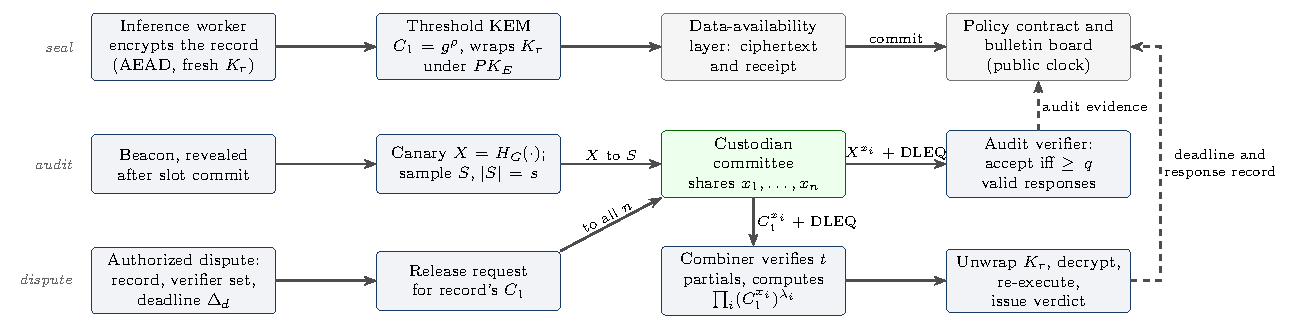
\includegraphics[width=\textwidth]{figures/fig1_architecture.pdf}
\caption{KEYSTONE architecture. Sealing, routine canary auditing and authorized dispute release are separate paths over one custodian committee. The audit uses a beacon-derived canary, never a production ciphertext; only an authorized dispute requests partial decryptions of a record's KEM component $C_1$. Dashed arrows are public evidence written to the bulletin board.}
\label{fig:architecture}
\end{figure*}

\subsection{Readiness and security properties}

For request type $u\in\{\mathsf{audit},\mathsf{dispute}\}$, $\mathsf{Ready}_i(E,\tau,u,\Delta)=1$ iff custodian $i$ can access its valid current share, execute the required operation, produce a valid proof and deliver its response by $\tau+\Delta$. Audit and dispute readiness differ on purpose: a target-aware custodian may answer a canary and refuse a particular dispute. Table~\ref{tab:properties} lists the properties and where this paper assesses each.

\begin{table}[t]
\centering
\caption{Properties separated by KEYSTONE, how each is assessed in this paper, and the evidence type.}
\label{tab:properties}
\small
\begin{tabularx}{\textwidth}{@{}>{\raggedright\arraybackslash}p{0.17\textwidth}X>{\raggedright\arraybackslash}p{0.25\textwidth}>{\raggedright\arraybackslash}p{0.17\textwidth}@{}}
\toprule
Property & Meaning & Assessed by & Evidence type\\
\midrule
Ciphertext availability ($\CA$) & Encrypted record and receipt bytes are retrievable from the DA layer & Assumed (provided by the DA layer); contrast class & Assumption\\
Valid-share registration & Registered shares are consistent with one epoch key (DKG/VSS/PVSS) & Feldman commitment checks at keygen & Prototype tests\\
Audit-time readiness ($\AKR$) & At least $q$ of $s$ sampled custodians return valid canary partials by the audit deadline & Eq.~\eqref{eq:hypergeom}; Tables~\ref{tab:robustness}, \ref{tab:acceptance} & Exact; simulation; emulation\\
Authorized decryptability & After authorization, the combiner obtains $t$ distinct valid partials of $C_1$ & Prototype open path; Table~\ref{tab:robustness} & Tests; emulation\\
Deadline liveness ($\DDL$) & Authorized decryptability completes by $\Delta_d$ & Figure~\ref{fig:deadline}; Table~\ref{tab:robustness}(b) & Single-host emulation\\
Pre-authorization confidentiality ($\PAC$) & With fewer than $t$ shares, an adversary learns nothing about $K_r$ beyond base-scheme leakage & Inherited from the threshold KEM \citep{boneh2006threshold}; canary never touches $C_1$ & Design argument\\
$(\varepsilon,\Delta_d)$-DKA & With probability $\geq 1-\varepsilon$ the combiner obtains $t$ valid partials by $\tau+\Delta_d$, and $\PAC$ holds before & Composition of the rows above & Conditional\\
\bottomrule
\end{tabularx}
\end{table}

\subsection{Adversaries and exclusions}

The model covers independent crash faults, provider, region or software-domain correlated outages, invalid or equivocal responses, changing compromise across epochs, selective withholding, beacon prediction or substitution, and unauthorized requests. Confidentiality assumes fewer than $t$ current shares are compromised. Production DKG/PVSS security, malicious authorized verifiers, arbitrary asynchronous partitions and fully adaptive selective-withholding resistance are out of scope. Invalid proofs and equivocation are positive cryptographic evidence; attributing a missed deadline to malice additionally requires the declared synchrony and delivery assumption.

\section{KEYSTONE Protocol}\label{sec:protocol}

\paragraph{Epoch setup and sealing.} The committee is formed under identity, stake and failure-domain placement policy. A production system would use an authenticated DKG or PVSS; the prototype uses a dealer with Feldman commitments \citep{feldman1987vss} as a substitution boundary. The worker encrypts the record under $K_r$, publishes $C_1=g^{\rho}$, derives $PK_E^{\rho}$ and uses it to wrap $K_r$. The envelope binds epoch, record identifier, ciphertext, metadata and DA pointer.

\paragraph{Non-production readiness audit.} The coordinator commits epoch and audit slot before the beacon is known. The finalized beacon then fixes a uniform or domain-stratified sample $S$ of size $s$, and all parties derive
\[
X=H_G(\texttt{KEYSTONE-CANARY}\parallel E\parallel \mathsf{slot}\parallel \mathsf{beacon}),
\]
where $H_G$ is domain separated and does not expose $\log_g X$. Sampled custodian $i$ returns $D_i=X^{x_i}$ with a Chaum--Pedersen proof that $\log_g Y_i=\log_X D_i$, bound to the request context \citep{chaum1992dleq,rfc9380}. The verifier checks membership, freshness, uniqueness, proof validity and deadline, and accepts after $q$ valid responses. Because $X$ is fresh and derived, the audit exercises share access without opening a production record, and a coordinator cannot substitute a record's $C_1$ as a challenge.

\paragraph{Authorized dispute release.} A dispute starts only after the policy contract binds a record, epoch, authorized verifier set and deadline. Custodians verify the authorization and return $C_1^{x_i}$ with a DLEQ proof. The combiner verifies $t$ distinct responses and interpolates in the exponent, $\prod_{i\in I}(C_1^{x_i})^{\lambda_i}=C_1^{x}=PK_E^{\rho}$, then unwraps $K_r$, decrypts and runs the authorized verification. The public transcript records valid, invalid, equivocal, stale, unauthorized and missing responses; plaintext release policy stays separate.

\section{Analysis}\label{sec:analysis}

\subsection{Static catastrophic false acceptance}

Let exactly $r<t$ custodians be audit-ready throughout one request. If $s$ custodians are sampled uniformly without replacement and acceptance requires $q$ valid responses,
\begin{equation}
\Pr[\mathsf{accept}\mid r]=\sum_{j=q}^{\min(s,r)}\frac{\binom{r}{j}\binom{n-r}{s-j}}{\binom{n}{s}}.
\label{eq:hypergeom}
\end{equation}
This is non-decreasing in $r$, so the worst catastrophic state is $r=t-1$, and for $q=s$
\begin{equation}
\varepsilon_a=\Pr[\mathsf{false\ accept}]\leq\frac{\binom{t-1}{s}}{\binom{n}{s}}.
\label{eq:bound}
\end{equation}
For $n=32$, $t=22$, $s=q=8$, $\varepsilon_a=0.0193462822$ and detection $1-\varepsilon_a=0.9806537178$. These are exact under the static model, not field-calibrated probabilities. If the catastrophic ready set is fixed and samples are independent and unpredictable, $m$ audits all falsely accept with probability at most $\varepsilon_a^m$; this does not hold for time-varying or adaptive readiness without a temporal model. Figure~\ref{fig:detection} shows how detection grows with $s$ and how the bound scales with committee size under $t=n-\lfloor(n-1)/3\rfloor$.

\begin{figure*}[t]
\centering
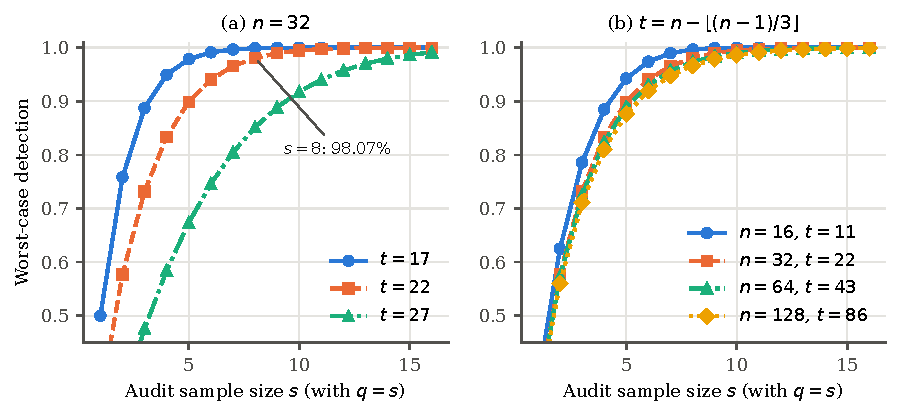
\includegraphics[width=\textwidth]{figures/fig2_detection_vs_sample.pdf}
\caption{Exact worst-case detection $1-\binom{t-1}{s}/\binom{n}{s}$ versus sample size with $q=s$. (a)~Thresholds $t\in\{17,22,27\}$ at $n=32$; the baseline $s=8$, $t=22$ is annotated. (b)~Committee sizes $16$--$128$. Values for $(n,s)\in\{(16,4),(32,8),(64,12),(128,16)\}$ are listed in Table~\ref{tab:scalability}.}
\label{fig:detection}
\end{figure*}

\subsection{Three non-implication witnesses}

\begin{enumerate}
  \item $\CA\not\Rightarrow\DKA$: ciphertext stays available while only $t-1$ custodians are dispute-ready.
  \item $\AKR\not\Rightarrow$ target-dispute success: selective custodians answer the canary and withhold the target response. With $w=n-t+1$ withholders the dispute fails deterministically while every audit passes (Figure~\ref{fig:withholding}).
  \item A finite sequence of accepted audits $\not\Rightarrow$ future $\DKA$: enough custodians may become unavailable after the last audit.
\end{enumerate}

\subsection{The acceptance-rule trade-off}

Requiring $q=s$ maximizes detection but turns every benign miss in the sample into an alarm. Under independent unavailability $f$, a healthy committee passes with probability $\Pr[\mathrm{Bin}(s,1-f)\geq q]$, which for $s=q=8$ and $f=0.10$ is only $0.43$ although $t$ of $32$ shares are almost surely reachable. Table~\ref{tab:acceptance} and Figure~\ref{fig:acceptance} give the exact trade-off. At $s=8$ no rule achieves both: $q=7$ lowers detection to \RAccEightSevenDet{} while benign pass rises to \RAccEightSevenPass{}. A larger sample recovers the trade-off: $s=16$, $q=14$ detects \RAccSixteenFourteenDet{} of worst-case catastrophic states with benign pass \RAccSixteenFourteenPassFive{} at $f=0.05$ and \RAccSixteenFourteenPassTen{} at $f=0.10$. This analysis was added after observing the high benign alarm rate in exploratory runs and is reported as design guidance, not as a prespecified result.

\begin{table}[t]
\centering
\caption{Exact acceptance-rule trade-off at $n=32$, $t=22$: worst-case catastrophic detection ($r=t-1$) versus the probability that a healthy committee passes under IID unavailability $f$. Post hoc analysis.}
\label{tab:acceptance}
\small
\begin{tabular}{@{}rrrrrr@{}}
\toprule
 & & Worst-case & \multicolumn{3}{c}{Benign audit pass under IID unavailability}\\
\cmidrule(lr){4-6}
$s$ & $q$ & detection & $f=0.05$ & $f=0.10$ & $f=0.20$\\
\midrule
8 & 6 & 57.5\% & 99.4\% & 96.2\% & 79.7\%\\
8 & 7 & 85.9\% & 94.3\% & 81.3\% & 50.3\%\\
8 & 8 & 98.1\% & 66.3\% & 43.0\% & 16.8\%\\
12 & 10 & 89.6\% & 98.0\% & 88.9\% & 55.8\%\\
12 & 11 & 98.2\% & 88.2\% & 65.9\% & 27.5\%\\
12 & 12 & 99.9\% & 54.0\% & 28.2\% & 6.9\%\\
16 & 13 & 93.2\% & 99.3\% & 93.2\% & 59.8\%\\
16 & 14 & 98.8\% & 95.7\% & 78.9\% & 35.2\%\\
16 & 15 & 99.9\% & 81.1\% & 51.5\% & 14.1\%\\
\bottomrule
\end{tabular}

\end{table}


\section{Evaluation}\label{sec:evaluation}

\subsection{Method and evidence labels}

Table~\ref{tab:config} lists every experiment. We separate four evidence types and label each result with one of them. \emph{Exact} values are closed-form under a declared model. \emph{Simulation} results come from three cells whose parameters, endpoints, precision targets and seed schedule were written and hashed before execution: 32 seed blocks of 4{,}096 independent draws each (131{,}072 draws per cell), which exceeds the Hoeffding requirement of 73{,}778 draws for the stated half-widths \citep{hoeffding1963}. The sampling-policy cell uses common random numbers, so uniform and stratified samples are compared on the same failure draw. \emph{Microbenchmarks} are single-process wall-clock medians. \emph{Emulation} is a testbed of 32 custodian operating-system processes on one host. Proportions carry 95\% Wilson intervals \citep{wilson1927}. The emulated testbed is not a geo-distributed deployment.

\begin{table}[t]
\centering
\caption{Experimental configuration. The baseline committee is $n=32$, $t=22$, $s=q=8$ with four failure domains of eight custodians.}
\label{tab:config}
\small
\begin{tabularx}{\textwidth}{@{}>{\raggedright\arraybackslash}p{0.2\textwidth}>{\raggedright\arraybackslash}p{0.3\textwidth}X@{}}
\toprule
Experiment family & Parameters & Execution and evidence label\\
\midrule
Static bound (Eq.~\ref{eq:bound}) & $n\in\{16,32,64,128\}$, $t=n-\lfloor (n-1)/3\rfloor$, $s\in\{1,\dots,16\}$, $q=s$; baseline $n=32,t=22,s=q=8$ & Exact closed form\\
PC03 prespecified cells & $n=32,t=22,s=q=8$, 4 domains of 8. IID: $p_{\mathrm{off}}=0.10$. STRAT: $p_{\mathrm{dom}}=0.20$, $p_{\mathrm{off}}=0.02$, uniform vs.\ 2-per-domain quota. SW: $w=11$ & 32 seed blocks $\times$ 4{,}096 draws $=131{,}072$ per cell; seeds frozen before execution; simulation\\
Correlation model & $f\in\{0,0.025,\dots,0.40\}$; IID vs.\ 2/4/8 equal domains & Exact; declared synthetic model\\
Acceptance rule & $s\in\{8,12,16\}$, $q\in[\lceil s/2\rceil,s]$, IID $f\in\{0.05,0.10,0.20\}$ & Exact; post hoc\\
Cryptographic cost & ffdhe2048, ffdhe3072 (RFC 7919) and the 256-bit prototype group; $n\le 128$ & Local microbenchmark, CPython 3.13, Apple M4 Pro\\
Deadline testbed & ffdhe2048, $n=32,t=22$; 8 profiles $\times$ 300 traces; one-way delay lognormal (median 0/40/120\,ms); 2\% loss; 10 or 11 crashes; one-domain outage; $\Delta_d\in\{0.25,0.5,1,2,5\}$\,s & 32 custodian processes on one host, loopback TCP, real cryptography; emulation\\
\bottomrule
\end{tabularx}

\end{table}

\begin{figure*}[t]
\centering
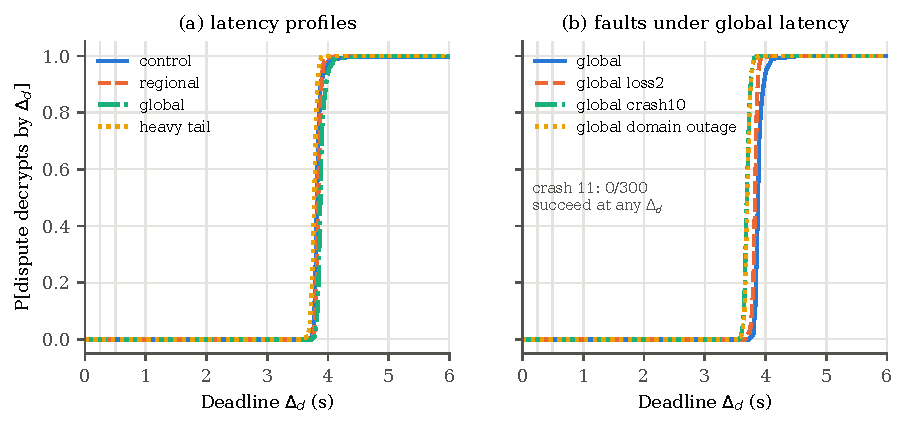
\includegraphics[width=\textwidth]{figures/fig3_dispute_success_vs_deadline.pdf}
\caption{Empirical probability that an authorized dispute decrypts the correct plaintext by deadline $\Delta_d$, single-host emulation with real ffdhe2048 cryptography, \RDLTraces{} traces per profile. (a)~Latency profiles. (b)~Faults under the 120\,ms-median profile; with eleven crashed custodians no dispute succeeds. Vertical lines mark the evaluated deadlines $0.25$, $0.5$, $1$, $2$ and $5$\,s.}
\label{fig:deadline}
\end{figure*}

\subsection{Comparison with readiness baselines}

Table~\ref{tab:baselines} compares the canary audit with the obvious alternatives. A heartbeat confirms only that a process responds; a custodian that has lost its share still answers, so a static catastrophic state of $t-1$ share-holders is invisible to it. Share registration is checked once and says nothing about later share loss. Decrypting a real record would test the right capability but discloses a production record. A full-committee canary probe detects every static catastrophic state at four times KEYSTONE's per-round cost at $n=32$; KEYSTONE trades that cost for the detection probability of Eq.~\eqref{eq:bound}.

\begin{table}[t]
\centering
\caption{Readiness checks compared. Costs are measured medians for ffdhe2048 in the prototype (Table~\ref{tab:operations}); bytes are canonical request plus response transcripts.}
\label{tab:baselines}
\small
\begin{tabularx}{\textwidth}{@{}>{\raggedright\arraybackslash}p{0.17\textwidth}>{\raggedright\arraybackslash}p{0.15\textwidth}>{\raggedright\arraybackslash}p{0.14\textwidth}>{\raggedright\arraybackslash}p{0.17\textwidth}X@{}}
\toprule
Readiness check & Exercises the secret share? & Touches production ciphertext? & Detects a static state with $r=t-1$ ready shares & Cost per check ($n=32$, ffdhe2048, measured)\\
\midrule
Liveness heartbeat & No & No & No: a node that lost its share still answers & 1 message per node; no group operations\\
Share registration (Feldman/PVSS check) & Once, at setup & No & No: says nothing about later share loss & One-time $O(nt)$ exponentiations at epoch setup\\
Full-committee canary probe & Yes & No (canary) & Yes, with probability 1 & 32 proofs + 32 verifications; 8501\,ms CPU; 36,991\,B\\
KEYSTONE sampled canary ($s=q=8$) & Yes, for the sampled members & No (canary) & Yes, with probability 0.9807 (Eq.~\ref{eq:bound}) & 8 proofs + 8 verifications; 2125\,ms CPU; 9,415\,B\\
Decrypt a real record as a test & Yes & Yes: exposes a production record & Yes & $t$ verifications plus a real disclosure; excluded by design\\
\bottomrule
\end{tabularx}

\end{table}

\subsection{Robustness under failure scenarios}

Table~\ref{tab:robustness}(a) reports the prespecified simulation cells. Under 10\% independent unavailability the committee reconstructs in \RIIDRecon{} of draws, yet the strict audit passes in only \RIIDAudit{}: the audit is a sensitive alarm, not an accurate health score. Under 20\% domain outages, fixed-quota stratified sampling raised conditional detection of catastrophic draws from \RStratDetU{} to \RStratDetS{} and lowered the benign pass rate from \RStratPassU{} to \RStratPassS{}. The prespecified primary endpoint, the paired difference in detected catastrophes per draw, was \RStratD{} (Hoeffding half-width \RStratHW{}; all \RStratDiscordant{} discordant pairs favored stratification), so stratification's benefit is real but small in this cell. With eleven selective withholders, audits passed in \RSWAudit{} of draws and disputes succeeded in \RSWDispute{} (upper 95\% bound \RSWDisputeHi{}), confirming the second non-implication witness at the prespecified sample size.

\begin{table}[t]
\centering
\caption{Robustness under failure scenarios. (a)~Prespecified simulation; dispute success equals reconstructability because the simulator has no network. (b)~Emulated testbed: audit pass is $q=8$ valid responses within the 6\,s timeout; dispute success requires correct plaintext within $\Delta_d=2$\,s; times are over successful disputes, from first request to decrypted plaintext.}
\label{tab:robustness}
\small
\begin{tabularx}{\textwidth}{@{}>{\raggedright\arraybackslash}X r r r r r@{}}
\toprule
Scenario & Audit pass & Dispute success & By $\Delta_d=5$\,s & Median time & p95 time\\
\midrule
\multicolumn{6}{@{}l}{\textit{(a) PC03 prespecified simulation, 131{,}072 draws per cell, 95\% Wilson intervals}}\\
IID 10\% unavailable & 43.1\% [42.8, 43.3] & 99.98\% [99.97, 99.99] & -- & -- & --\\
Domain outage 20\%, uniform sample & 37.3\% [37.0, 37.6] & 81.3\% [81.1, 81.6] & -- & -- & --\\
Domain outage 20\%, stratified sample & 34.9\% [34.7, 35.2] & 81.3\% [81.1, 81.6] & -- & -- & --\\
11 selective withholders & 100.0\% [99.997, 100.000] & 0.0\% [0.000, 0.003] & -- & -- & --\\
\addlinespace
\multicolumn{6}{@{}l}{\textit{(b) Emulated deadline testbed, ffdhe2048; dispute success by the primary $\Delta_d=2$\,s and by 5\,s, 95\% Wilson intervals}}\\
control & 100.0\% [98.7, 100.0] & 0.0\% [0.0, 1.3] & 99.7\% & 3818\,ms & 3936\,ms\\
regional & 100.0\% [98.7, 100.0] & 0.0\% [0.0, 1.3] & 100.0\% & 3841\,ms & 3908\,ms\\
global & 100.0\% [98.7, 100.0] & 0.0\% [0.0, 1.3] & 100.0\% & 3875\,ms & 4016\,ms\\
global loss2 & 71.7\% [66.3, 76.5] & 0.0\% [0.0, 1.3] & 100.0\% & 3829\,ms & 3886\,ms\\
global crash10 & 2.3\% [1.1, 4.7] & 0.0\% [0.0, 1.3] & 100.0\% & 3692\,ms & 3775\,ms\\
global crash11 & 1.7\% [0.7, 3.8] & 0.0\% [0.0, 1.3] & 0.0\% & -- & --\\
global domain outage & 5.7\% [3.6, 8.9] & 0.0\% [0.0, 1.3] & 100.0\% & 3700\,ms & 3780\,ms\\
heavy tail & 98.3\% [96.2, 99.3] & 0.0\% [0.0, 1.3] & 100.0\% & 3772\,ms & 3850\,ms\\
\bottomrule
\end{tabularx}

\end{table}

Figure~\ref{fig:correlation} shows why placement matters. At equal per-unit unavailability $f=0.10$, an IID committee reconstructs with probability \RIIDReconTen{}, four domains of eight (each under the placement cap $n-t=10$) with \RDomFourRecon{}, and two domains of sixteen, which violate the cap, with only \RDomTwoRecon{}. These are exact values under a declared synthetic model; real domain labels and their independence are assumptions.

\begin{figure*}[t]
\centering
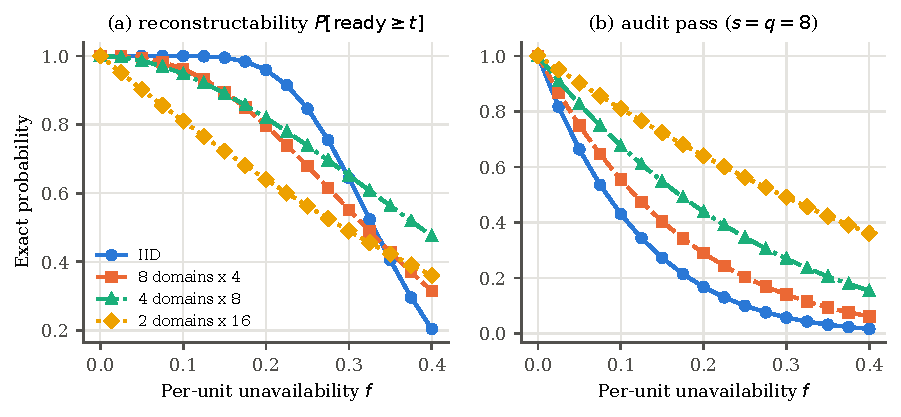
\includegraphics[width=\textwidth]{figures/fig4_iid_vs_correlated.pdf}
\caption{IID versus domain-correlated unavailability at $n=32$, $t=22$. A domain fails with probability $f$ and takes all its members; in the IID model each custodian fails independently with probability $f$. (a)~Reconstructability. (b)~Audit pass with $s=q=8$. Exact; a 20{,}000-draw Monte Carlo check agrees within $0.009$.}
\label{fig:correlation}
\end{figure*}

\begin{figure}[t]
\centering
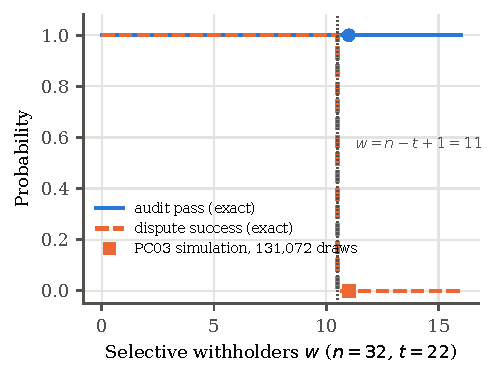
\includegraphics[width=0.6\textwidth]{figures/fig5_audit_vs_dispute_withholding.pdf}
\caption{Audit pass versus dispute success as the number of selective withholders $w$ grows, with no other failures. Lines are exact; markers at $w=11$ are the prespecified 131{,}072-draw simulation cell.}
\label{fig:withholding}
\end{figure}

\subsection{Deadline liveness in an emulated testbed}

The testbed runs 32 custodian processes, each an asyncio TCP server holding only its own ffdhe2048 share, and one combiner on the same host. Each trace performs one canary audit and one authorized dispute over a freshly sealed 1\,KiB record. The combiner verifies each DLEQ proof on arrival, stops at $t=22$ valid partials, combines, unwraps $K_r$ and checks the decrypted plaintext. One-way delays are drawn per message from a lognormal law with the profile's median; loss drops a message with no retransmission; crashed custodians never answer. Each of eight profiles ran \RDLTraces{} traces with seeds fixed before execution.

Figure~\ref{fig:deadline} and Table~\ref{tab:robustness}(b) report the results. The prespecified primary endpoint, success by $\Delta_d=2$\,s, was $0\%$ in every profile: no dispute finished in under 3.5\,s. Every reconstructable dispute finished within 5\,s, with medians from \RDLMedLo{} to \RDLMedHi\,s and a slowest success of \RDLMaxSucc\,s. Completion time is dominated by computation, not by the network. With no injected delay the median is \RDLControlMed\,ms, close to 22 serial proof verifications at the \RVerifyTwoK\,ms measured in Table~\ref{tab:operations}; adding a 120\,ms-median one-way delay moved the median only to \RDLGlobalMed\,ms, because responses arrive while the combiner is still verifying earlier ones. A heavy-tailed delay law ($\sigma=1.2$) did not lengthen completion (95th percentile \RDLHeavyTailPninefive\,ms). Ten crashes (median \RDLCrashTenMed\,ms) and a full domain outage (median \RDLDomainOutMed\,ms) completed slightly faster than the fault-free global profile, which we attribute to fewer custodian processes competing for the shared host CPU. Eleven crashes defeated every dispute (\RDLCrashElevenSucc{} succeeded).

The audit side reproduces Eq.~\eqref{eq:hypergeom} on real cryptography. A single audit took \RDLAuditMedLo--\RDLAuditMedHi\,s at the median. With ten crashed custodians the strict audit passed in \RDLCrashTenAudit{} of traces against an exact expectation of \RExpCrashTen{}; with one domain down, \RDLDomainOutAudit{} against \RExpDomainOut{}; with 2\% message loss, \RDLLossAudit{} against \RExpLoss{}. In the crash and outage profiles the dispute nevertheless succeeded in every trace, the benign-alarm pattern of Section~\ref{sec:analysis}. One control trace timed out because the combiner was slowed by unrelated activity on the shared host; it is counted as a failure.

The design implication is that $\Delta_d$ must budget for verifying $t$ proofs at the combiner. We did not measure optimized, batched or parallel verification, which would shorten this term.


\begin{figure}[t]
\centering
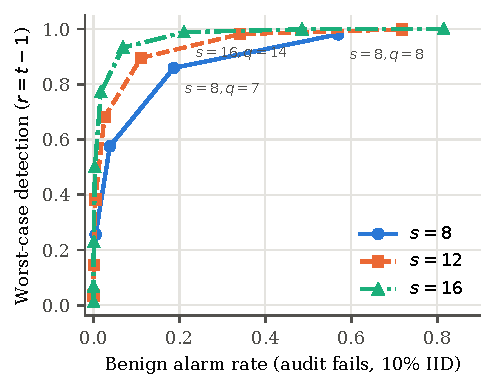
\includegraphics[width=0.62\textwidth]{figures/fig6_acceptance_tradeoff.pdf}
\caption{Detection versus benign alarm rate (audit fails while the committee is healthy, $f=0.10$) for each acceptance threshold $q$; one curve per sample size. Exact values from Table~\ref{tab:acceptance} and its full source grid.}
\label{fig:acceptance}
\end{figure}

\subsection{Performance and scalability}

Table~\ref{tab:operations} gives per-operation costs in the pure-Python prototype; these are upper bounds, and optimized libraries are substantially faster. At ffdhe2048 a custodian's partial decryption with proof takes \RProveTwoK\,ms and its verification \RVerifyTwoK\,ms; verifying 22 partials and combining takes \RCombineTwoK\,ms (\RCombineThreeK\,ms at ffdhe3072). The 256-bit prototype group is listed for reference only and is not a secure size. Table~\ref{tab:scalability} scales the committee: audit cost grows with $s$, not $n$, while dispute cost grows with $t$. Table~\ref{tab:gas} reports the bulletin-board gas costs measured in the Foundry harness.

\begin{table}[t]
\centering
\caption{Scalability with $t=n-\lfloor(n-1)/3\rfloor$. Detection is exact (Eq.~\eqref{eq:bound}, $q=s$). Audit CPU is $s$ proofs plus $s$ verifications; bytes are one request plus $s$ responses. Dispute time is measured verification of $t$ partials plus combination.}
\label{tab:scalability}
\small
\begin{tabular}{@{}rrrrrrrr@{}}
\toprule
 & & & & \multicolumn{2}{c}{Audit, ffdhe2048} & \multicolumn{2}{c}{Dispute: verify $t$ + combine}\\
\cmidrule(lr){5-6}\cmidrule(lr){7-8}
$n$ & $t$ & $s$ & Detection & CPU & Bytes & ffdhe2048 & ffdhe3072\\
\midrule
16 & 11 & 4 & 88.46\% & 1063\,ms & 4,819 & 1585\,ms & 5040\,ms\\
32 & 22 & 8 & 98.07\% & 2125\,ms & 9,415 & 3213\,ms & 10201\,ms\\
64 & 43 & 12 & 99.66\% & 3188\,ms & 14,011 & 6230\,ms & 20086\,ms\\
128 & 86 & 16 & 99.92\% & 4250\,ms & 18,607 & 12534\,ms & 40201\,ms\\
\bottomrule
\end{tabular}

\end{table}

\begin{table}[t]
\centering
\caption{Median wall time per operation, CPython 3.13 on an Apple M4 Pro; RFC~7919 groups \citep{rfc7919} with $q=(p-1)/2$ and generator~4. Pure-Python reference implementation.}
\label{tab:operations}
\small
\begin{tabular}{@{}lrrr@{}}
\toprule
Operation (median, ms) & 256-bit prototype & ffdhe2048 & ffdhe3072\\
\midrule
Canary derivation $H_G$ & 0.08 & 16.99 & 54.32\\
Partial decryption + DLEQ proof & 0.58 & 130.30 & 420.54\\
DLEQ verification & 0.75 & 135.36 & 430.58\\
Seal 1\,KiB record & 0.22 & 48.32 & 156.48\\
Partial response size (bytes) & 253 & 1149 & 1661\\
\bottomrule
\end{tabular}

\end{table}

\begin{table}[t]
\centering
\caption{Bulletin-board gas per operation, re-measured for this revision with Foundry 1.5.1 and Solidity 0.8.24 (test-body gas; fixture setup excluded). Each operation was measured in the small harness committee named in the scope column; values are deterministic and identical to the earlier snapshot.}
\label{tab:gas}
\small
\begin{tabularx}{\textwidth}{@{}l r X@{}}
\toprule
Bulletin-board operation & Gas & Harness scope\\
\midrule
Register epoch & 223,629 & n=5, t=3; duplicate-identity validation enabled\\
Open audit & 125,107 & three sampled members; q=3\\
Submit audit response & 57,882 & first commitment from one sampled custodian\\
Mark invalid response & 27,704 & admin records a non-zero evidence hash\\
Record equivocation & 51,710 & second conflicting commitment from one custodian\\
Finalize audit & 29,142 & two responses for a three-member sample after deadline\\
Open dispute & 144,149 & n=5, t=3; all members eligible\\
Cancel request & 5,709 & admin cancels one open audit\\
\bottomrule
\end{tabularx}

\end{table}

\section{Discussion}

Availability is layered. Data availability answers whether encrypted bytes can be retrieved; share registration whether a key was formed consistently; a readiness audit whether sampled custodians can now perform a non-production share operation; an authorized dispute whether $t$ custodians will serve a specific target before a deadline. Treating these as interchangeable hides distinct failure modes, and the evaluation shows each one separating in practice: high reconstructability with low audit pass under benign failures, perfect audit pass with zero dispute success under selective withholding, and dispute completion governed by verification work at the combiner rather than by average network latency.

Three design consequences follow. First, the acceptance rule should be chosen for a target benign alarm rate, which in our analysis favors larger samples with $q<s$ over $s=q$. Second, failure-domain placement under the cap $n-t$ matters more than sampling policy: violating the cap cost far more reconstructability than stratification changed detection. Third, deadlines must budget for verifying $t$ proofs at the combiner; in our prototype that term exceeded the injected network delay by more than an order of magnitude. Non-response proves absence from the transcript, not malice, so penalties should distinguish warning, temporary inactivity, replacement and slashing.

\section{Limitations}

\begin{enumerate}
  \item \textbf{Novelty.} Broad component novelty is defeated by prior work; the narrow composition has not been independently reviewed for novelty.
  \item \textbf{Future cooperation.} The audit does not prove it; selective withholding is a counterexample, not a solved problem.
  \item \textbf{Temporal inference.} Repeated-audit multiplication requires a static ready set or a justified temporal model.
  \item \textbf{Emulation, not deployment.} The deadline testbed runs on one host with loopback TCP and synthetic delay laws; geo-distributed behavior, congestion and clock skew are not measured, and host scheduling caused one control-trace timeout. Completion times reflect a pure-Python implementation and would differ for optimized code.
  \item \textbf{Non-production prototype.} A dealer replaces DKG/PVSS; the pure-Python code and the bulletin-board contract have not been externally audited.
  \item \textbf{Post hoc analysis.} The simulation design was prespecified and hashed before execution; one analysis (Table~\ref{tab:acceptance}) was added afterwards and is labeled post hoc.
  \item \textbf{External validity.} Failure models are synthetic; no claim is made about real provider, region or operator behavior.
\end{enumerate}
The hypothesis should be rejected or reframed if a predecessor already makes the same dispute-specific property and readiness probe explicit, or if independent reproduction fails to recover the property separations reported here.

\section{Conclusion}

KEYSTONE isolates a failure mode that ciphertext data availability does not address: the threshold service needed for an authorized encrypted-rollup dispute may be unavailable, slow or uncooperative at the deadline. It decomposes the relevant properties, instantiates a non-production canary audit from established components, and gives an exact static detection bound. The evaluation shows that the audit detects catastrophic states, that its acceptance rule needs tuning to avoid benign alarms, that it cannot detect selective withholding, and that in an emulated 32-custodian committee every reconstructable dispute completes within five seconds, a budget set by proof verification rather than by the network. KEYSTONE measures present sampled serviceability under declared assumptions; it does not prove future availability or introduce a new threshold-decryption primitive.

\section*{Declarations}

\textbf{Study type and ethics.} Non-human computational research using synthetic data, simulation, locally generated prototype outputs and smart-contract tests; no personal data, participants, production secrets or live systems.

\textbf{Data and code availability.} Source code, frozen designs with SHA-256 hashes, seed schedules, raw per-block and per-trace outputs, and the scripts that generate every table and figure are publicly available at \url{https://github.com/zmzubraj/KeyStone} under the MIT License.

\textbf{Funding and conflicts of interest.} This work was self-funded. The author declares no conflicts of interest.

\textbf{AI-assisted preparation.} AI assistance was used for drafting, code integration, experiment scripting and figure generation. The author is responsible for the scientific content, verification and submission.

\bibliographystyle{unsrtnat}
\bibliography{references_r1}

\end{document}
